\section{POODLE as the Main Case Study}

POODLE stands for \emph{Padding Oracle On Downgraded Legacy Encryption}. The attack became public in 2014 and demonstrated that SSL 3.0 was no longer acceptable for modern secure communication. Its importance goes beyond one protocol version. POODLE showed how an old protocol, compatibility fallbacks, and CBC padding behavior can combine into a practical attack against real users.

The key setting was the downgrade path. Many clients and servers still supported SSL 3.0 for backward compatibility, and some clients would fall back to SSL 3.0 if earlier handshake attempts failed. A man-in-the-middle attacker could interfere with the connection, trigger the fallback, and force the victim to communicate under SSL 3.0. Once that happened, the attacker could exploit SSL 3.0's CBC record processing.

The SSL 3.0 design was especially weak because the padding bytes were not constrained the way later TLS versions intended. In SSL 3.0, only the padding length byte had a strict meaning, while the other padding bytes could be arbitrary. As a result, a modified record could accidentally satisfy the padding format with probability about $1/256$ for a targeted byte. That probability is small for a single attempt but becomes practical when the attacker can trigger many repeated requests carrying a secret such as a session cookie.

\begin{figure}[H]
    \centering
    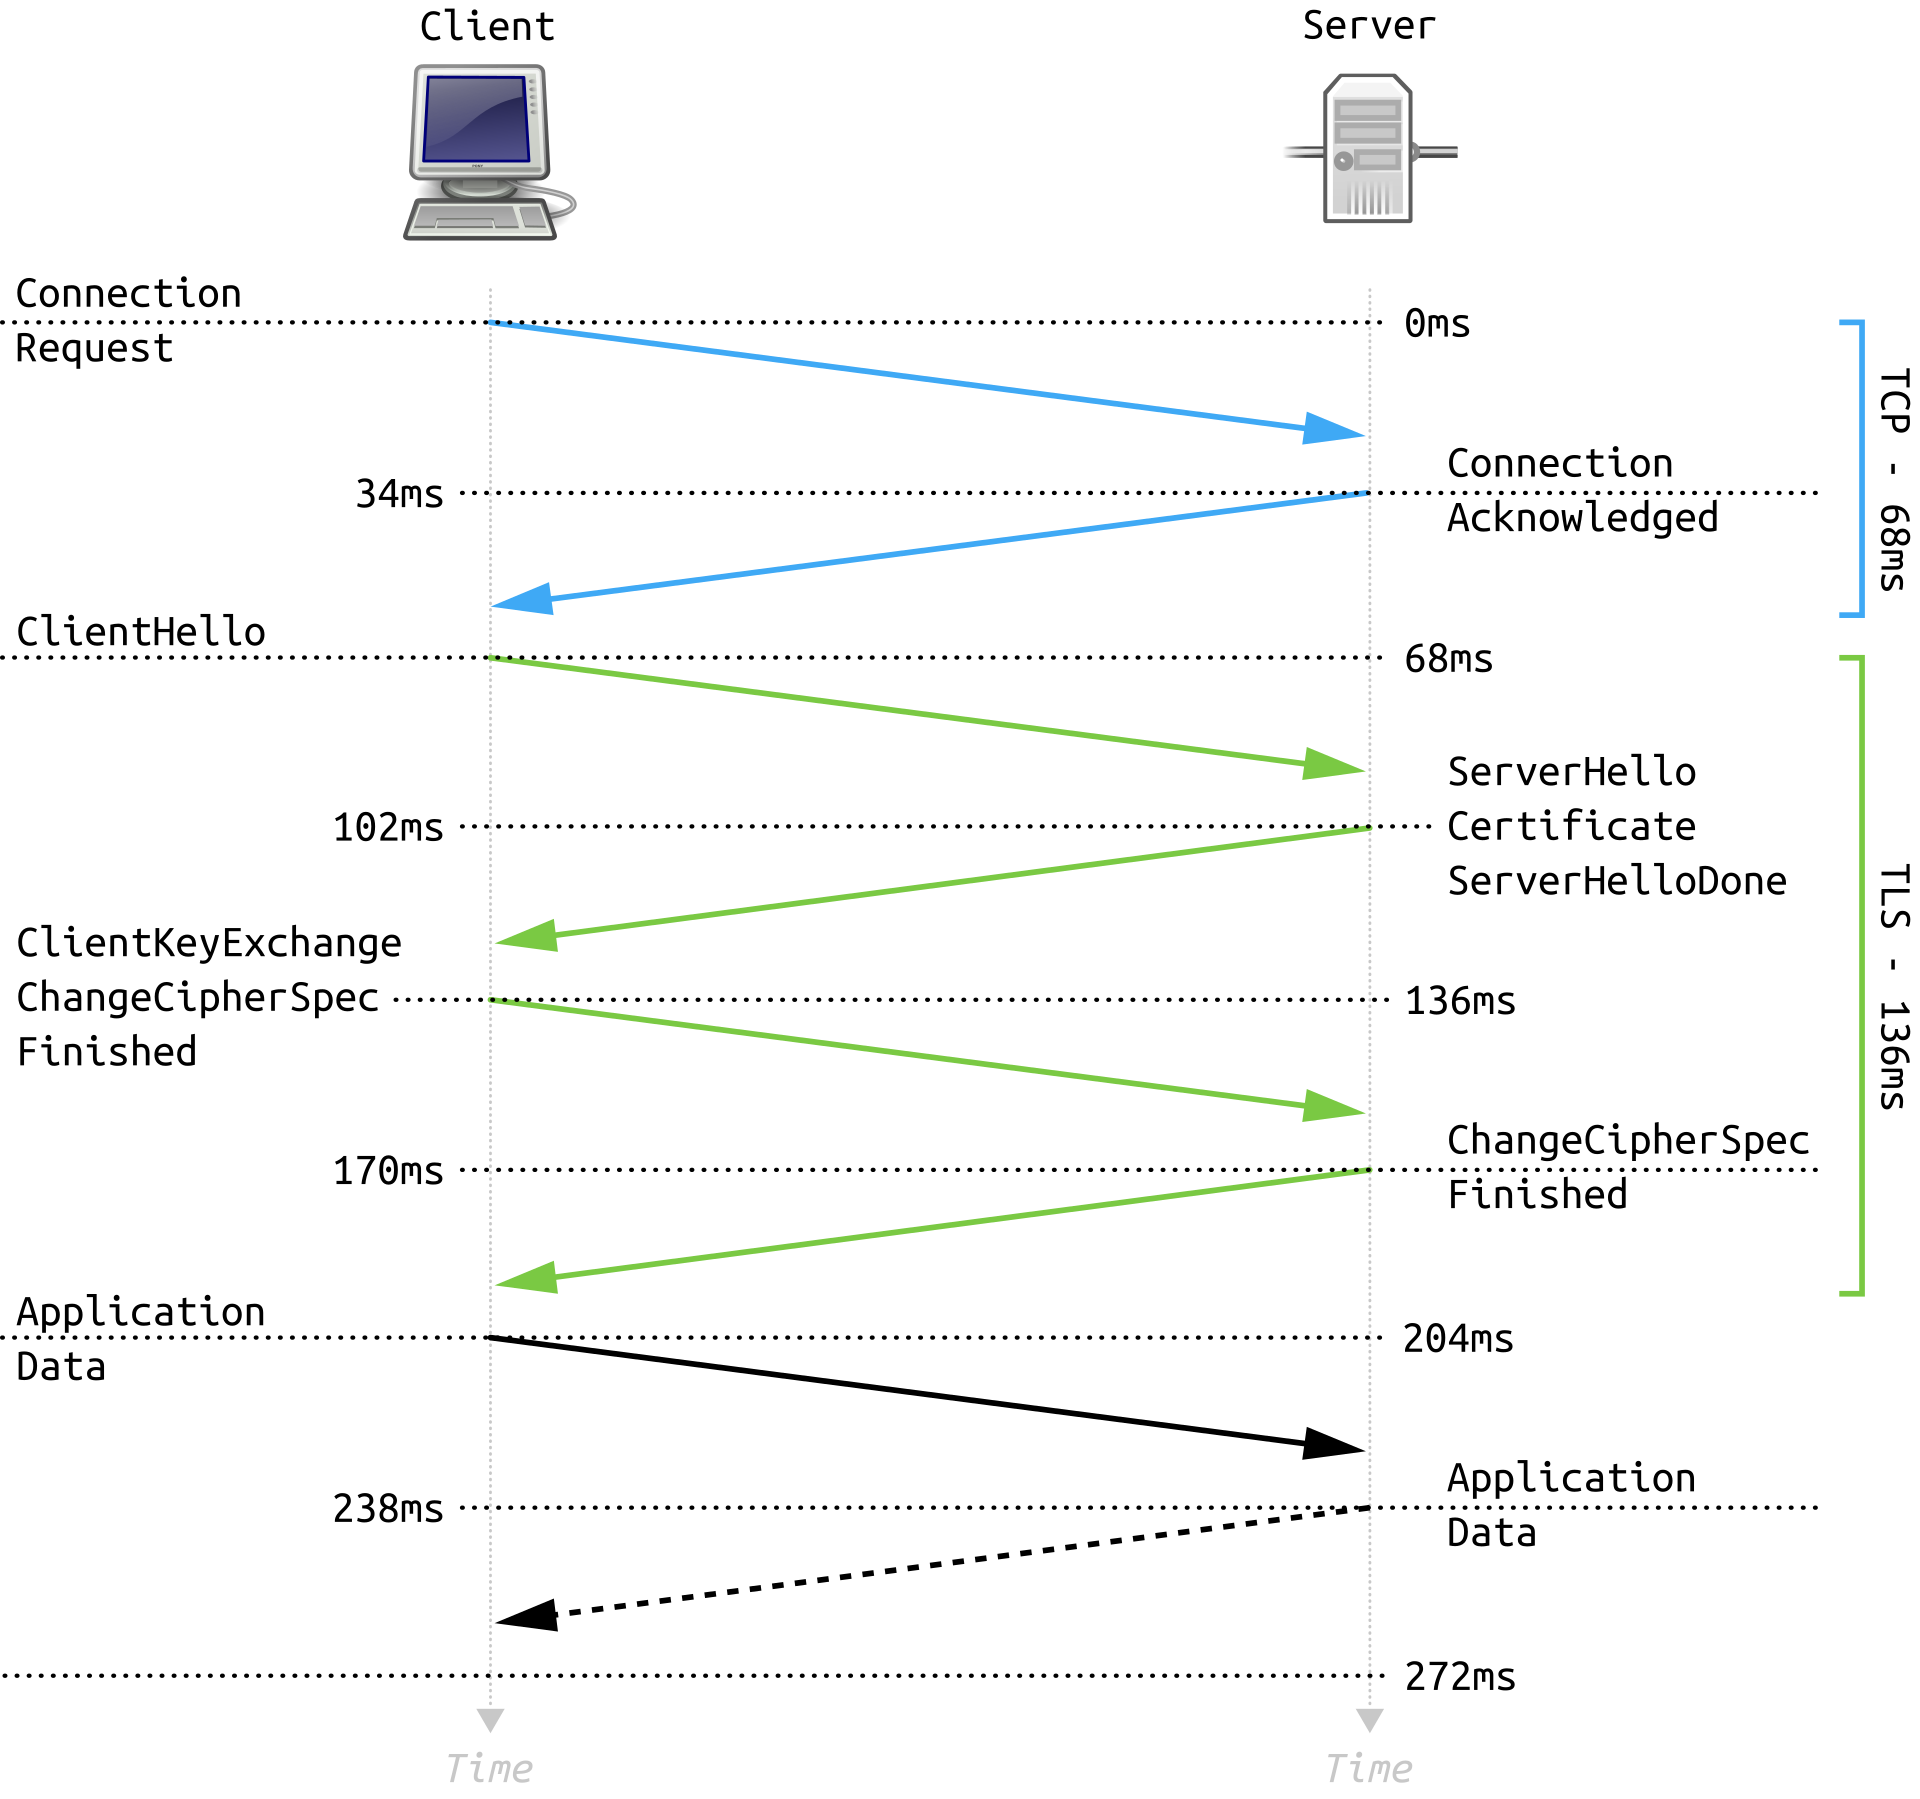
\includegraphics[width=0.78\textwidth]{images/tls12_handshake.png}
    \caption{Handshake message flow in the TLS protocol family. POODLE targeted the older SSL 3.0 branch of this protocol line through downgrade and CBC-padding weaknesses.}
    \caption*{\footnotesize Source: Wikimedia Commons, \emph{Full TLS 1.2 Handshake.svg}.}
    \label{fig:ssl-simple}
\end{figure}

The attack workflow can be summarized as follows:

\begin{enumerate}
    \item the attacker forces a downgrade from a newer protocol to SSL 3.0,
    \item the attacker causes the victim to send repeated requests containing a secret value,
    \item the attacker manipulates ciphertext blocks in those requests, and
    \item the server's acceptance or rejection of the padding reveals one byte of information at a time.
\end{enumerate}

POODLE therefore turned a theoretical padding oracle into a network attack against web traffic. It also changed operational practice. After the disclosure, major vendors disabled SSL 3.0 support, and the IETF formally deprecated SSL 3.0. The lesson was not only that legacy protocols are dangerous, but also that backward-compatibility paths can revive vulnerabilities long after the community believes it has moved on.

It is important to distinguish POODLE from the local Python demonstration in this project. The project code demonstrates the \emph{generic padding oracle mechanism}: forged ciphertext, padding validation, and byte-by-byte plaintext recovery. POODLE adds protocol-specific details such as downgrade behavior, repeated browser requests, and SSL 3.0 record semantics. The mathematical core is shared, but the surrounding attack environment is richer in the real protocol case.
